\documentclass[conference]{IEEEtran}
\IEEEoverridecommandlockouts
\usepackage{cite}
\usepackage{amsmath,amssymb,amsfonts}
\usepackage{algorithmic}
\usepackage{graphicx}
\graphicspath{{img/}}
\usepackage{textcomp}
\usepackage[table]{xcolor}
\usepackage{verbatim}
\usepackage{tabularx}
\def\BibTeX{{\rm B\kern-.05em{\sc i\kern-.025em b}\kern-.08em
    T\kern-.1667em\lower.7ex\hbox{E}\kern-.125emX}}
\begin{document}



\title{
 Cosmic\\Design Report}

\author{\IEEEauthorblockN{Clay Buxton}
\IEEEauthorblockA{\textit{Computer Engineering, Computer Science} \\
\textit{Elizabethtown College}\\
Elizabethtown, PA \\
buxtonc@etown.edu}
\and
\IEEEauthorblockN{Kevin Carman}
\IEEEauthorblockA{\textit{Computer Engineering, Computer Science} \\
\textit{Elizabethtown College}\\
Elizabethtown, PA \\
carmank@etown.edu}

}

\maketitle

\section{Design Methodology}
\subsection{Overview}
Cosmic is a fully emulated, lightweight, and cross-platform 8-bit computer architecture with a RISC-like instruction set designed alongside a rich GUI interface to test, debug, and run the system.

\subsection{Development}
Before any development of Cosmic began, in-depth research was conducted on processors of the time period, like the Z80 and 6502, to build a feature set that would satisfy the goals we wanted to achieve. We documented how other processors implemented various addressing modes and instructions and how other similar projects implemented their solutions in software.

After everything was mapped out and planned, development began simultaneously with the creation of the GUI interface environment and the backbone code of the processor itself. The GUI was developed to allow for easy debugging throughout the design process and for usability of the final project. At first, it was designed to include nothing but a hex editor, a display for the registers, program counter, and stack pointer, and three buttons to cycle the program counter and reset the processor and memory. The backbone code was made up of two files, a header file and a class file. The header file housed the function prototypes, type declarations, registers, program counter, and stack pointer. The class file defined the functions for fetching, decoding, and executing along with the various addressing types we planned to implement. It was set up to allow for easy implementation of instructions as development carried on.

We worked together for a short time putting some finishing touches on the design and implementing a few opcodes, but split up to work more efficiently. Kevin focused on implementing and testing all of the opcodes for the processor while Clay moved on to start writing the assembler.

The Cosmic assembler is close to done, but requires a little more development to work out the kinks. All the opcodes thus far have been implemented and tested except for the recent addition of interrupt handling. In the upcoming weeks we plan to finish the assembler and to implement unit testing for all the opcodes which means we are right on schedule with what we believed we could achieve this semester.

\subsection{Workflow}
\begin{figure}[h!]
	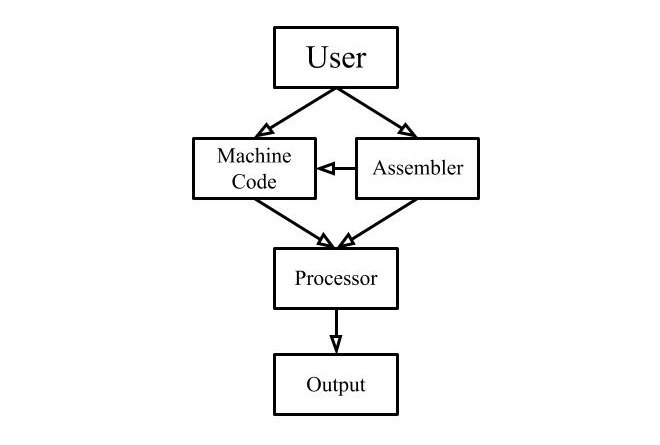
\includegraphics[width=\linewidth]{block_dia.jpg}
	\caption{The Cosmic workflow.}
	\label{fig:The Cosmic Workflow}
\end{figure}

The block diagram in Figure \ref{fig:The Cosmic Workflow} shows the path the user can follow to input their program, run the processor, and obtain the results. Once the user has the GUI up and running, they can input a program written in either assembly or machine code. If the user opts to write their program in assembly, then it will be converted to machine code so that the Cosmic processor can understand it. Currently, the user must manually step the processor to run through their program, but a method to automatically step will be implemented soon. The output of the program is wherever the user specifies it to be, either storing it in memory or leaving it in one of the registers. This is subject to change once we develop the I/O capabilities of Cosmic.

\subsection{Results}


\section{Design Choices}
\subsection{Bitness}
The "bitness" of a chip is traditionally the size of the data bus. An 8-bit chip can address 8 bits of data at one time, a 16-bit chip can address 16 bits of data etc.

Our design choice was between an 8-bit design and a 16-bit design. 32-bit and 64-bit designs were not considered as they did not exist during the time that the chips that Cosmic is similar to were made.\\

\resizebox{\columnwidth}{!}{%
 \begin{tabular}{||c|c|c|c|c||}
 \hline
 Factors & Practical Use & Implementation & Appropriate Design & \cellcolor{blue!40}Total\\ [0.5ex] 
 \hline\hline
 Weights & 3 & 2 & 2& \\ 
 \hline
 8-bit & 5 &  8&  9 & \cellcolor{blue!25}49\\
 \hline
 16-bit  &  8 & 5 &  5 & \cellcolor{blue!25}44\\
 \hline
\end{tabular}
}\\

An 8-bit chip was chosen mainly due to it being more relevant to the class of chips Cosmic is made to fit in with, those of the early 80's and late 70's. A 16-bit chip would have been slightly more work to implement, but would have been much more useful to write for.

\subsection{Registers vs. Zero Page vs In-Memory Registers}

Chips of the time generally had registers in 3 formats. There were many registers separated from memory like in the Z80. Few registers and then an easily accessible portion of memory like in the 6502. Or on chips with on-board memory, the registers would take up the first few bytes of memory.

Each of these has it's pros and cons, but all configurations were designed with two things in mind, speed and utility. On a physical chip, retrieving data from a register is significantly faster than a location in memory, but you only had 8 bytes. Getting something from zero page memory on the 6502 was faster than getting something from another place in memory, but slower than a register, but you had 256 bytes.\\

\resizebox{\columnwidth}{!}{%
 \begin{tabular}{||c|c|c|c|c||}
 \hline
 Factors & Practical Use & Implementation & Appropriate Design & \cellcolor{blue!40}Total\\ [0.5ex] 
 \hline\hline
 Weights & 3 & 2 & 2& \\ 
 \hline
 Many Registers & 9 &  8&  10 & \cellcolor{blue!25}63\\
 \hline
 Zero Page  &  5 & 5 &  10 & \cellcolor{blue!25}45\\
 \hline
 Onboard Memory &  6 & 10 &  7& \cellcolor{blue!25}52\\

 \hline 
\end{tabular}
}\\

Registers, similar to the Z80 made the most sense in our case. Since there is no speed difference between accessing zero page and accessing any other position in memory in our design, zero page addressing would be a waste of time to implement. On-board memory would have been very easy to develop, but was generally found on microcontrollers rather than microprocessors, and would have held no real speed boost either.

\subsection{16-Bit Register Mode}
16-bit register mode is when two of the 8-bit registers can be used together to act as a 16-bit register. This can also be done for certain instructions as well.\\

\resizebox{\columnwidth}{!}{%
 \begin{tabular}{||c|c|c|c|c||}
 \hline
 Factors & Practical Use & Implementation & Appropriate Design & \cellcolor{blue!40}Total\\ [0.5ex] 
 \hline\hline
 Weights & 3 & 2 & 2& \\ 
 \hline
 No 16 Bit mode & 4 &  8&  10 & \cellcolor{blue!25}48\\
 \hline
 16 Bit mode &  10 & 6 &  10 & \cellcolor{blue!25}62\\
 \hline
\end{tabular}
}\\

Overall, a 16-bit mode was a good decision. This allows for a lot more usability, and still fits in with chips of the time since the Z80 also had 16-bit mode instructions. This did add a bit of work, significantly increasing our instruction count,  but was worth it overall.

\subsection{Signed vs. Unsigned Data}

During the design we were unsure how to use signed and unsigned numbers. In the Z80 and 6502 there is no distinction between the two in position of memory since the arithmetic functions do binary math. The programmer must keep track of if the number is signed or unsigned and flags are used in math to signify certain cases.\\

\resizebox{\columnwidth}{!}{%
 \begin{tabular}{||c|c|c|c|c||}
 \hline
 Factors & Practical Use & Implementation & Appropriate Design & \cellcolor{blue!40}Total\\ [0.5ex] 
 \hline\hline
 Weights & 3 & 2 & 2& \\ 
 \hline
 Specifically Signed Data & 8 &  4 &  3 & \cellcolor{blue!25}38\\
 \hline
 Overflow and Carry flags &  5 & 8 &  7 & \cellcolor{blue!25}45\\
 \hline
\end{tabular}
}\\

While having specifically signed functions and locations would have been helpful, it would have been a lot to implement and not really consistent with how processors work. Instead we focused on having flags when using arithmetic functions show if things would be negative and when it would overflow.

\subsection{Op-code Selection}

The op-code selection is the control logic of a simulated chip. It takes an op-code in from memory and has to resolve it to a instruction to execute. This can be done in a few ways. One way is using a large switch statement to branch to the proper instruction function. This can be large and cumbersome, but is also very simple. Another way is to use function pointers and then store them in a way in which they can be easily called. We could also create a struct to hold the function pointer and then other things relevant to the instruction like size, mnemonic, and addressing mode.\\

\resizebox{\columnwidth}{!}{%
 \begin{tabular}{||c|c|c|c|c||}
 \hline
 Factors & Practical Use & Implementation & Appropriate Design & \cellcolor{blue!40}Total\\ [0.5ex] 
 \hline\hline
 Weights & 3 & 2 & 2& \\ 
 \hline
 Switch Statement & 3 & 10& n/a& \cellcolor{blue!25}29\\
 \hline
 Function Pointers &  7& 7&  n/a& \cellcolor{blue!25}35\\
 \hline
 Function Pointers w/ Data &  9 & 7 &  n/a & \cellcolor{blue!25}41\\
 \hline
\end{tabular}
}\\

A switch statement is very large and cumbersome and also is a very crude way to select op-codes. We decided using an array of structs containing the function pointers, and additional data about the function way the best way to go. While it was tricky to implement, it works very well, is much faster than a switch statement, and also contains a lot of data about each of the functions. The instructions are put into an array at the position that their op-code is. For instance the NOP instruction is op-code 0x00, so it was put into the first element of the array so when InstructionSet[0] is called, it will return the struct which contains the function pointer for the NOP instruction

\subsection{Addressing functions}

When writing the functions for the op-codes, we were unsure on how to implement the addressing modes. They could either be done as separate functions or each instruction could be implemented separately with its addressing mode.\\

\resizebox{\columnwidth}{!}{%
 \begin{tabular}{||c|c|c|c|c||}
 \hline
 Factors & Practical Use & Implementation & Appropriate Design & \cellcolor{blue!40}Total\\ [0.5ex] 
 \hline\hline
 Weights & 3 & 2 & 2& \\ 
 \hline
 Individual Functions & 3 &  7&  n/a & \cellcolor{blue!25}23\\
 \hline
 Addressing Functions &  7 & 6 &  n/a & \cellcolor{blue!25}33\\
 \hline
\end{tabular}
}\\

Implementing each function with each addressing mode was very cumbersome as it increased the number of instruction functions significantly. Although 2 different functions have to be written for each function due to the way our addressing works, it reduced the total number of functions and made writing the remaining functions very easy. 

\subsection{GUI back-end}

The GUI back-end for the simulation environment was the smallest design decision to make. The main decision had to be made between immediate or a retained mode GUI. Qt4 ,a retained mode GUI and ImGUI, a immediate mode GUI were both libraries we were familiar with and could easily implement. \\

\resizebox{\columnwidth}{!}{%
 \begin{tabular}{||c|c|c|c|c||}
 \hline
 Factors & Practical Use & Implementation & Appropriate Design & \cellcolor{blue!40}Total\\ [0.5ex] 
 \hline\hline
 Weights & 3 & 2 & 2& \\ 
 \hline
 ImGui & 8 &  5&  n/a & \cellcolor{blue!25}34\\
 \hline
 Qt4 &  6 & 5 &  n/a & \cellcolor{blue!25}23\\
 \hline
\end{tabular}
}\\

We chose immediate mode due to how much would be changing on screen at a time, and since the elements in the GUI would not be super intensive, and ImGui is much easier to implement and works cross platform with few external dependencies.




\subsection{Supported Systems}

Targeting all operating systems can be difficult since they all require different dependencies and have different ways to build the software. macOS and Linux work similarly enough for our purposes and very few changes have to be made to the build process between macOS and Linux. Windows however requires a different process and generally requires tools installed that most people will not unless they are writing in C/C++ without Microsoft tools. \\

\resizebox{\columnwidth}{!}{%
 \begin{tabular}{||c|c|c|c|c||}
 \hline
 Factors & Practical Use & Implementation & Appropriate Design & \cellcolor{blue!40}Total\\ [0.5ex] 
 \hline\hline
 Weights & 3 & 2 & 2& \\ 
 \hline
 Windows, macOS, \& Linux & 8 &  5 &  n/a & \cellcolor{blue!25}34\\
 \hline
 macOS \& Linux &  6 & 7 &  n/a & \cellcolor{blue!25}32\\
 \hline
\end{tabular}
}\\

We ended up "supporting" windows. There are instructions and a makefile for building on windows, we currently have no good way of consistently testing and ensuring quality on Windows. While it works we do not officially support it and won't change things for the program to work better on Windows. 


\section{System Level Design}

The system currently consists of 2 source files, envmain.cpp, and cosproc.cpp. Envmain holds all of the GUI code and also acts as a motherboard to the processor right now along with "fake" memory since the memory class has not yet been implemented. Eventually, the motherboard part of the code will be moved into its own class, but since we don't have any other system parts developed, it worked well for the testing environment. Cosproc is the processor itself and works very similarly to a 6502 or Z80. Internally it has registers, a program counter, and all the other components of a processor. An assembler, separate to the rest of the project, is written in Python and called cosasm.py. 

The figure below gives a brief overview over the current and near-future design of the cosmic system, with the elements in dotted outlines not yet being implemented.

\begin{figure}[h!]
	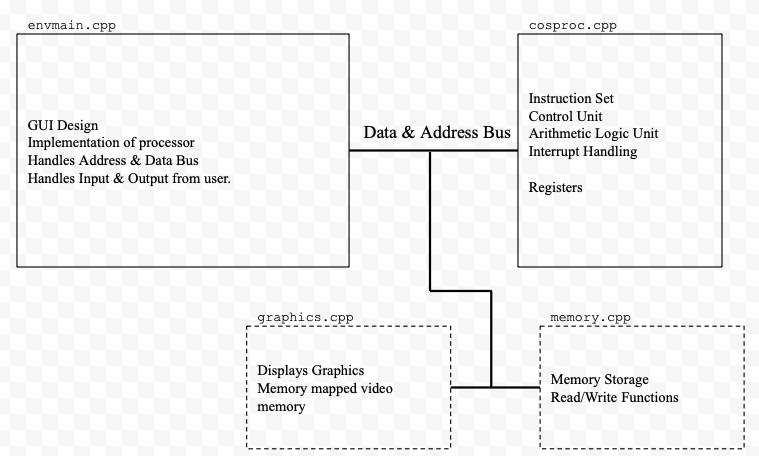
\includegraphics[width=\linewidth]{SystemDesign.png}
	\caption{The Cosmic workflow.}
	\label{fig:The Cosmic Workflow}
\end{figure}



\subsection{Environment Main [envmain.cpp]}

The environment main holds the initialization of ImGUI, SDL, and OpenGL, alongside building the GUI elements. This is all constructed in the main ImGui loop. As previously mentioned envmain also currently acts as a motherboard for the system, holding a 64Kb byte array, which acts as the memory and the MemoryWrite and MemoryRead functions that serve as a Data and Address bus. The GUI currently shows the status of the internal registers, a control panel for stepping and resetting the processor, and a memory editor that displays and allows editing of all addressable memory. 


\subsection{Cosmic Processor [cosproc.cpp]}

The cosmic processor is a standalone processor that can technically be implemented anywhere and does not rely on the environment main to work. The processor was designed to function similarly to a real processor. On every cycle, the processor goes through the same sequence. Read from memory, decode the instruction, and execute the instruction. The processor itself does not know anything other than the instruction it is currently executing. In code, the opcode is read, and it decoded by checking the InstructionSet array that holds all of the addressing modes, instruction function, size, and mnemonic for each opcode. Once the addressing mode and opcode function have been retrieved, the addressing mode function is executed to find the operand in memory. This location is passed to the opcode function, which then does whatever the instruction entails.


\subsection{Cosmic Assembler [cosasm.py]}

The cosmic assembler takes in assembly code and translates it to binary, which the processor can read. The assembly language has some support for things like variables, labels, and constants, but it very simple at the moment. The assembler does two passes through the assembly code, first to find all of the variables and put them at the head of the binary, then goes line by line and translates instructions into binary code.


\subsection{Memory, Video, and Other Planned System Components}
In the near future many more components to the cosmic system are planned. The two most significant are memory and video. Memory is mainly to properly implement a memory module instead of it being a massive array in the environment's main class. The second is video output. Video is all memory-mapped, which means a position in memory will represent an element on the screen. This is a simplistic approach to video output and is similar to older systems.

Down the line, time permitting, we also want to implement other things like sounds, emulated expansions, and other devices common on physical machines. 


\end{document}